\documentclass[aspectratio=43]{beamer}

%%% Beamer options
\usetheme{Dresden}
\usecolortheme{beaver}
% remove the navigation buttons from the lower right
\beamertemplatenavigationsymbolsempty
% show slide numbers
\setbeamertemplate{footline}[frame number]

% error when symbols are not found in a font (since no font-fallback seems to exist)
% \tracinglostchars=3

\usepackage{amsmath}
\usepackage{amssymb}
\usepackage{amsfonts}
\usepackage{mathtools}
\usepackage{fontspec}
\usepackage{minted}
\usepackage{todonotes}
\usepackage{newunicodechar}
\usepackage{graphicx}
\usepackage{mathpartir}

\setmonofont{Source Code Pro}
\newfontfamily\symfont{FreeMono}
\newfontfamily\symfontextra{FreeSerif}

% define some unicode characters missing from Source Code Pro
\newunicodechar{∗}{{\symfont ∗}}
\newunicodechar{⊥}{{\symfont ⊥}}
\newunicodechar{▷}{{\symfont ▷}}
\newunicodechar{↦}{{\symfont ↦}}
\newunicodechar{∨}{{\symfont ∨}}
\newunicodechar{∈}{{\symfont ∈}}


\newcommand{\ocaml}[1]{\mintinline{ocaml}{#1}}
\newcommand{\coq}[1]{\mintinline{coq}{#1}}
\newcommand{\ocf}{OCaml~5}
\newcommand{\done}{{\symfontextra ✓}}
\newcommand{\tbd}{{\symfontextra ⌛}}
\newcommand{\wand}{-\kern-.6em\raisebox{-.659ex}{*}\ }
\newcommand{\efork}{\ocaml{Fork}}
\newcommand{\esuspend}{\ocaml{Suspend}}
\newcommand{\egetctx}{\ocaml{GetContext}}
\newcommand{\proto}{\mathtt{Coop}}
\newcommand{\ewp}[3]{\textit{ewp}\; #1\; \langle #2 \rangle\; \{#3\}}
\newcommand{\pers}[1]{\Box\; #1}
\newcommand{\pinv}{\textit{promiseInv}}

\title{Verifying an Effect-Based Cooperative Concurrency Scheduler in Iris}
\author{Adrian Dapprich\newline Advisors: Prof. Derek Dreyer \& Prof. François Pottier}
\institute{Dreyer Laboratory, MPI-SWS, Saarland University}
\date{22. September 2023}

\begin{document}

\frame{\titlepage}

\section{Introduction}

\begin{frame}{Self Introduction}
    \begin{itemize}
        \item Adrian Dapprich, master student and also former bachelor student at Saarland University.
        \item Interest in Iris and program verification after taking the Semantics lecture.
        \item Just finished an exchange year at Tohoku University at the lab of Prof. Sumii.
    \end{itemize}
\end{frame}

\begin{frame}{Today's Topic}
    \begin{itemize}
        \item Recently \ocf{} released with support for effect handlers.
        \item Eio is a multi-threaded, cooperative concurrency library for \ocf{} built around effects.
        \item Hazel\footnote{[Paulo de Vilhena. 2022]} is an implementation of a language with effect handlers in Iris.
        \item[\(\Rightarrow\)] We want to verify (a part of) the Eio library using Hazel to show the \textbf{safety} and \textbf{effect safety} of its central abstractions.
    \end{itemize}
\end{frame}

\begin{frame}{Why Eio?}
    \begin{itemize}
        \item Eio might replace previous concurrency libraries.
        \item Effects are more composable than monads, so easier to use than monadic-style concurrency libraries like \texttt{Lwt} and \texttt{Async}.
        \item Effects can be more efficient than monadic-style coding because it uses continuations for control flow instead of repeated bind operations.
    \end{itemize}
\end{frame}

\begin{frame}{Why Hazel?}
    \begin{itemize}
        \item Eio uses the CQS\footnote{[Nikita Koval et al. 2023]. Already verified in Iris but Eio uses a customized variant which we want to verify.} lock-free datastructure for cross-thread communication.
        \item Eio uses effects handlers for implementing cooperative concurrency.
        \item Hazel provides a framework for carrying out separation logic proofs about an ML-like language with effect handlers in Iris.
        \item[\(\Rightarrow\)] A perfect match!
    \end{itemize}

\end{frame}

\section{Background}

\begin{frame}[fragile]{Effect Handlers Example}
    \begin{minted}[highlightlines={8},fontsize=\footnotesize]{ocaml}
type _ Effect.t += Get : unit -> int Effect.t
type _ Effect.t += Put : int -> unit Effect.t

let get () = perform (Get ())
let put v = perform (Put v)

let client () = 
  run ~init:0 (fun () ->
    for i = 0 to 5 do
      let x = get () in
      put (x + i)
    done;
    get ())

(* > client ();;
   => 15 *)
\end{minted}
\end{frame}

\begin{frame}[fragile]{Effect Handlers Example}
    \begin{minted}[highlightlines={2,10,12},fontsize=\footnotesize]{ocaml}
let run ~init f =
  let rec loop : type a r. int -> (a, r) continuation -> a -> r =
    fun state k x ->
      continue_with k x
      { retc = (fun result -> result);
        exnc = raise;
        effc = (fun (type b) (eff: b Effect.t) ->
          match eff with
          | Get () -> Some (fun (k: (b,r) continuation) ->
              loop state k state)
          | Put v -> Some (fun (k: (b,r) continuation) ->
              loop v k ())
          | _ -> None)
      }
  in
  loop init (fiber f) ()
\end{minted}
\end{frame}

\begin{frame}[fragile]{Effect Handlers}
    \begin{itemize}
        \item Separate the code performing an effect from the code implementing an effect.
        \item Performing an effect captures a continuation up to the handler, aka "resumable exceptions".
        \item A form of "delimited continuation" but easier to understand than \textit{shift/reset} etc.
        \item \ocf{} supports effect handlers but without an effect system. Programs are not "effect-safe", i.e. there can be unhandled effects.
    \end{itemize}
\end{frame}

\begin{frame}{Eio}
    \begin{itemize}
        \item Concurrency library for \ocf{} using the new effect handlers.
        \item Abstractions over OS resources like filesystem, network, etc.
        \item Synchronization constructs like mutexes, semaphores, etc.
        \item Intends to be the main concurrency library for \ocf{}, replacing earlier \texttt{Async} and \texttt{Lwt}.
    \end{itemize}
\end{frame}


\begin{frame}{Eio}
    \begin{columns}
        \begin{column}{0.5\textwidth}
            \begin{itemize}
                \item \ocaml{Fiber} represents a concurrent computation.
                \item \ocaml{Scheduler} runs \ocaml{Fiber}s in one thread and handles their effects.
                \item \ocaml{CQS} is used to implement synchronization constructs for multi-threading.
                \item \ocaml{Cancel} implements \ocaml{Fiber} cancellation.
                \item \ocaml{Switch} is used for scoped resource control.
            \end{itemize}
        \end{column}
        \begin{column}{0.5\textwidth}
            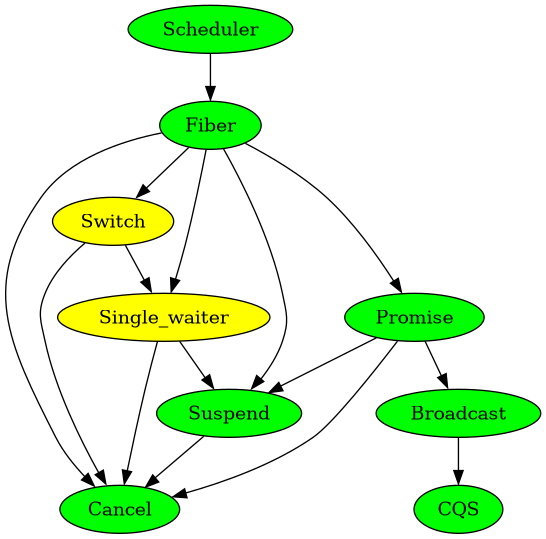
\includegraphics[width=\textwidth]{codept}
        \end{column}
    \end{columns}
\end{frame}

\begin{frame}{Hazel}
    \begin{itemize}
        \item Implementation of a language with effect handlers in Iris.
        \item Extended WP with protocols\footnote{Inspired by formalization of session types.} that define which effects can be performed during evaluation.
        \item Existing case studies about control inversion \& cooperative concurrency
        \item No multi-threading support and no atomic expressions defined.
        \item No type system but effect-safety is proved by extended WP.
    \end{itemize}
    \begin{align*}
        \text{Protocols:}   & \quad \Psi \Coloneqq \bot \mid\; !\; \vec{x}\; (v)\; \{ P \}.\; ?\; \vec{y}\; (w)\; \{ Q \} \\
        \text{Extended WP:} & \quad \ewp{\texttt{e}}{\Psi}{w.\; Q}
    \end{align*}
\end{frame}

\section{Contribution}

\begin{frame}{Plan}
    Build an extended cooperative concurrency case study based on Eio using Hazel.
    \begin{itemize}
        \item Three effects are used to communicate between fibers and their scheduler: \ocaml{Fork}, \ocaml{Suspend} \& \ocaml{GetContext}
        \item Fibers can await other fibers using promises (built on \ocaml{CQS}).
        \item Fibers can use OS resources
        \item Fibers can be cancelled which signals them to stop and prevents OS resource usage.
        \item[]
        \item Fibers and resources are registered to switches. If all fibers have exited, the resources can be cleaned up.
        \item Switches are organized in a hierarchy and you can cancel whole subtrees.
    \end{itemize}
\end{frame}

\begin{frame}{Plan}
    Build an extended cooperative concurrency case study based on Eio using Hazel.
    \begin{itemize}
        \item[\done{}] Simple cooperative concurrency scheduler using Eio effects, handling of promises in the fibers \& an axiomatization of CQS.
        \item[\done{}] Proof-of-concept for the \texttt{GetContext} effect.
        \item[\done{}] Definition of atomic expressions in Hazel.
        \item[\tbd{}] Add multi-threading to Hazel.
            \begin{itemize}
                \item[\tbd{}] Add support for the \texttt{iInv} tactic to Hazel.
            \end{itemize}
        \item[\tbd{}] Use a smaller axiomatization of CQS.
            \begin{itemize}
                \item[\tbd{}] Ideally, port CQS development to Hazel and remove axioms.
            \end{itemize}
        \item[\tbd{}] Verify example client program that uses threads \& fibers.
    \end{itemize}
\end{frame}

\begin{frame}{Contribution}
    Let us look at an example interaction between the cooperative concurrency scheduler and a fiber performing an async computation.
\end{frame}

\begin{frame}[fragile]{Client Fiber}
    Start two async network requests and wait for their completion (using the low-level API).
    \begin{minted}{ocaml}
let main () = 
    let p1 = fork_promise fetch_api in
    let p2 = fork_promise fetch_api in
    let r1 = await p1 in 
    let r2 = await p2 in 
    r1 + r2
\end{minted}
\end{frame}

\begin{frame}[fragile]{Specifications}
    \begin{mathpar}
        %     promiseInv ∗ EWP (f #()) <| Coop  |> {{v, □ Φ v}}
        %   ⊢ 
        %     EWP (fork_promise f) <| Coop  |> {{ y, 
        %       ∃ (p: loc), ⌜ y = #p ⌝ ∗ isPromise p Φ }}.
        % \inferrule [Fork]
        % {\pinv{} \ast \ewp{f\; ()}{\proto{}}{v.\; \pers{\Phi\; v}}}
        % {\ewp{\texttt{fork_promise f}}{\proto{}}{p.\; \textit{isPromise}\; p\; \Phi}}

        % \and

        % promiseInv ∗ isPromise p Φ ⊢ 
        %   EWP (await #p) <| Coop |> {{v, □ Φ v}}.
        % \inferrule [Await]
        % {\pinv{} \ast \textit{isPromise}\; p\; \Phi}
        % {\ewp{\texttt{await p}}{\proto{}}{v.\; \pers{\Phi\; v}}}
        % 
        % \and
        % 
        %   let P := (λ v, ⌜ v = #() ⌝ ∗ promise_state_done γ)%I in
        %     isMember p γ ε ∗ isPromiseResult ε Φ ∗ promise_cqs wakers γ
        %   ⊢
        %     EWP (await_callback #p wakers) <| ⊥ |> {{f, 
        %       ∀ (waker: val), (∀ (v: val), P v -∗ EWP (waker v) <| ⊥ |> {{_, True }}) -∗
        %       promiseInv -∗ 
        %         (▷ EWP (f waker) <| ⊥ |> {{_, True }}) }}.
        % \inferrule [Await-Callback]
        % {\textit{isMember}\; p\; \gamma\; \epsilon \ast \textit{isPromiseResult}\; \epsilon\; \Phi \ast \textit{promiseCqs}\; cqs\; \gamma}
        % {\ewp{\texttt{await\_callback}\; p\; cqs}{\bot}{f. \forall waker.\; I \ast  }}

        % \and
        % promiseInv -∗
        %   (promiseInv -∗ EWP main #() <| Coop |> {{ v, □ Φ v }}) -∗
        %     EWP run main {{ _, True }}.
        % \inferrule [Run]
        % {\pinv{} \ast (\pinv{} \wand{} \ewp{\texttt{main ()}}{\proto{}}{\top})}
        % {\ewp{\texttt{run main}}{\bot}{\top}}

    \end{mathpar}
\end{frame}


\begin{frame}[fragile]{Source Code}
    \begin{columns}[t]
        \begin{column}{0.4\textwidth}
            \begin{minted}[fontsize=\footnotesize]{ocaml}
let fork f =
  let p = new_promise () in
  fork (fun () ->
    let v = f () in
    match !p with
    | Done _ -> raise Error 
    | Waiting q -> 
      p := Done v;
      Cqs.resume_all q
  );
  p
\end{minted}
        \end{column}
        \begin{column}{0.5\textwidth}
            \begin{minted}[fontsize=\footnotesize]{ocaml}
let await p =
  match !p with
  | Done v -> v
  | Waiting q ->
    suspend (fun waker ->
      let req = Cqs.suspend q waker in
      match !p with
      | Done _ -> 
        Cqs.cancel cqs req; 
        waker ()
      | Waiting _ -> ()
    );
    match !p with
    | Done v -> v
    | Waiting _ -> raise Error
\end{minted}
        \end{column}
    \end{columns}
\end{frame}


\begin{frame}[fragile]{Source Code}
    \begin{minted}[fontsize=\footnotesize]{ocaml}
type 'a waker = 'a -> unit
type 'a suspender = 'a waker -> unit
type _ Effect.t += Fork : (unit -> unit) -> unit t
type _ Effect.t += Suspend : 'a suspender -> 'a t

let rec fulfill: (unit -> unit) -> unit = fun e ->
   match_with e () {
     effc = fun eff ->
       match eff with
       | Fork f -> Some (fun k ->
           Queue.add (fun () -> continue k ()) q;
           fulfill f)
       | Suspend suspender -> Some (fun k -> 
           let waker = fun v -> Queue.add (fun () -> continue k v) q in
           suspender waker;
           next ())
   }
    \end{minted}
\end{frame}

\begin{frame}[fragile]{Ghost State}
    \begin{minted}{coq}
Definition promise_cqs (wakers: val) (γ : gname) : iProp Σ :=
  is_cqs wakers (λ waker, ∀ (v: val), promise_state_done γ -∗
            EWP (waker v) <| ⊥ |> {{_, True }} ).
  
Definition promiseInv_inner : iProp Σ := (
  ∃ M, isPromiseMap M ∗ 
    [∗ map] args ↦ tt ∈ M, let '(p, γ, ε) := args in
      ((* Fulfilled: *) ∃ y,
        p ↦ Done' y ∗ promise_state_done γ ∗ 
        ∃ (Φ: val -d> iPropO Σ), isPromiseResult ε Φ ∗ □ Φ y)
    ∨
      ((* Unfulfilled: *) ∃ wakers,
        p ↦ Waiting' wakers ∗
        promise_state_waiting γ ∗
        promise_cqs wakers γ)).
\end{minted}
\end{frame}

\begin{frame}[fragile]{Proof of \ocaml{await}}
    a
\end{frame}

\begin{frame}{Contribution}
    Proof-of-concept for the \texttt{GetContext} effect.
    \todo[inline]{TODO Protocol with gname parameter and example how GetContext can be used}
\end{frame}

\begin{frame}{A note on cancellation}
    \begin{itemize}
        \item Eio has a mechanism for cancelling fibers.
        \item We tried to define a suitable specification for cancelled fibers.
              \begin{itemize}
                  \item A cancelled fiber cannot use any OS resources.
                  \item So we verify that the history of OS resource usage of a fiber does not grow after cancellation.
              \end{itemize}
        \item But fibers can become "protected" and be free of the restrictions of cancellation.
        \item Fibers can even protect themselves after noticing they are cancelled.
        \item Therefore, cancellation is just a signalling mechanism without any enforcable and thus verifiable behavior.
    \end{itemize}
\end{frame}

\section{Conlusion}
\begin{frame}{Tentative Evaluation}
    \begin{itemize}
        \item Our case study shows that an Eio-like scheduler with \efork{}, \esuspend{} \& \egetctx{} effects makes sense.
        \item We aim to show that it uses CQS correctly as a synchronization primitive.
        \item Real Eio has more ways of forking fibers and a hierarchy of cancellation contexts, which can be protected from cancellation. This part is not modelled.
    \end{itemize}
\end{frame}

\begin{frame}{Summary}
    \begin{itemize}
        \item We have finished a simple scheduler case study approximating Eio using the \efork{} \& \esuspend{} effects.
        \item Separately, we have mechanized the \egetctx{} effect to get meta-data about the current fiber.
        \item Next, we want to iteratively extend the case study to arrive at a more sizeable subset of Eio.
    \end{itemize}
\end{frame}

\section{Misc}

\begin{frame}[fragile]{Control flow in the protocol for \esuspend{}}
    \begin{itemize}
        \item \(P\; v\) appears in the precondition of \ocaml{waker}, which invokes the continuation.
        \item Therefore, we can prove \(P\; v\) in the postcondition of the protocol.
        \item \(P\; v\) allows us to conclude in \ocaml{promise_await} that the promise is fulfilled after performing the \esuspend{} effect.
    \end{itemize}
    \begin{align*}
        \textit{isSuspender}\; f\; \Coloneqq & \; \forall \textit{waker}.\; I \wand{}                                                                            \\
                                             & \quad (\forall v.\; P\; v \wand{} \textit{ewp}\; (\textit{waker}\; v)\; \langle \bot \rangle\; \{\top \}) \wand{} \\
                                             & \quad \triangleright \textit{ewp}\; (f\; waker)\; \langle \bot \rangle\; \{ \top \}                               \\
        \textit{SUSPEND}\;         \Coloneqq & \; !\; f\; P\; (f)\; \{ I \ast \textit{isSuspender}\; f \}.                                                       \\
                                             & \;?\; v\; (v) \{ P\; v \}
    \end{align*}
\end{frame}


\begin{frame}{Fiber-local storage}
    \begin{itemize}
        \item Eio supports fiber-local storage that can be queried by the \texttt{GetContext} effect.
        \item Authoritative ghost map in the scheduler to save the storage \(\bullet [\texttt{gname} \mapsto (\textit{Var} \to \textit{Val})]\).
        \item If we specify the gohst name that identifies the storage of a fiber in either the request or answer variables of the protocol, one party has an existentially quantified ghost name and cannot do anything with it.
        \item Therefore, we parameterize the whole protocol by the ghost name.
        \item That way both the handler and the handlee know which storage is accessible to the fiber.
    \end{itemize}
\end{frame}

\begin{frame}{Hazel Reasoning Rules}
    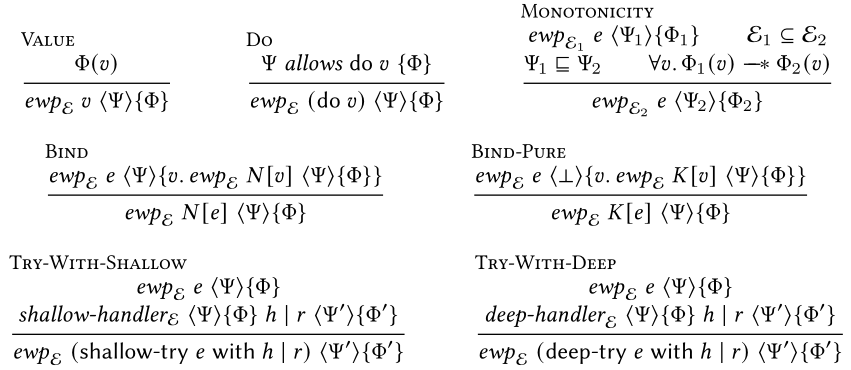
\includegraphics[width=\textwidth]{reasoning_rules1.png}
\end{frame}

\begin{frame}{Hazel Reasoning Rules}
    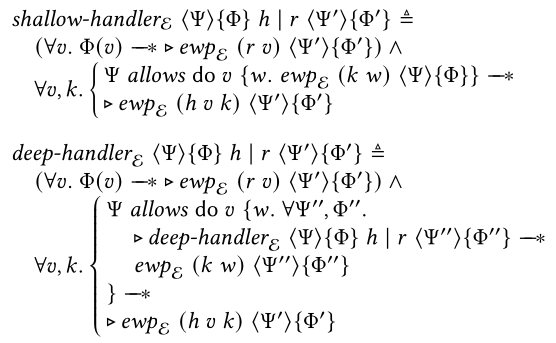
\includegraphics[width=\textwidth]{reasoning_rules2.png}
\end{frame}

\end{document}